\documentclass[14pt]{extbook}
\usepackage{multicol, enumerate, enumitem, hyperref, color, soul, setspace, parskip, fancyhdr} %General Packages
\usepackage{amssymb, amsthm, amsmath, latexsym, units, mathtools} %Math Packages
\everymath{\displaystyle} %All math in Display Style
% Packages with additional options
\usepackage[headsep=0.5cm,headheight=12pt, left=1 in,right= 1 in,top= 1 in,bottom= 1 in]{geometry}
\usepackage[usenames,dvipsnames]{xcolor}
\usepackage{dashrule}  % Package to use the command below to create lines between items
\newcommand{\litem}[1]{\item#1\hspace*{-1cm}\rule{\textwidth}{0.4pt}}
\pagestyle{fancy}
\lhead{Progress Quiz 6}
\chead{}
\rhead{Version C}
\lfoot{4563-7456}
\cfoot{}
\rfoot{Summer C 2021}
\begin{document}

\begin{enumerate}
\litem{
Choose the graph of the equation below.\[ f(x) = \frac{-1}{(x + 1)^2} - 1 \]\begin{enumerate}[label=\Alph*.]
\begin{multicols}{2}\item 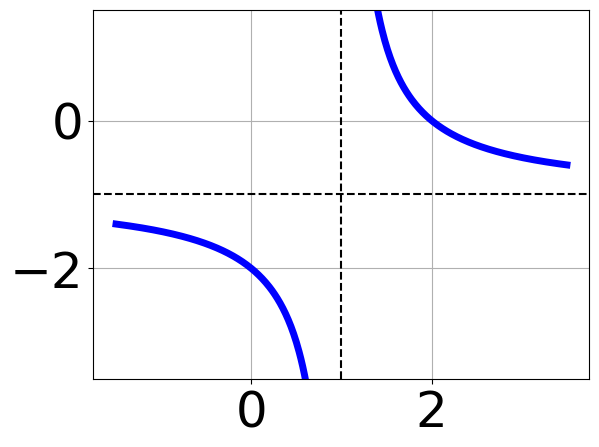
\includegraphics[width = 0.3\textwidth]{../Figures/rationalEquationToGraphAC.png}\item 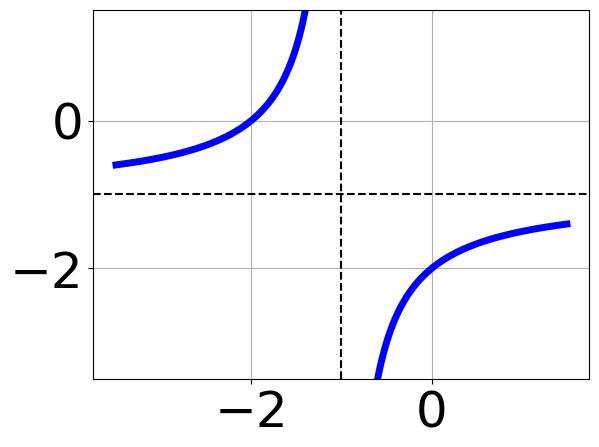
\includegraphics[width = 0.3\textwidth]{../Figures/rationalEquationToGraphBC.png}\item 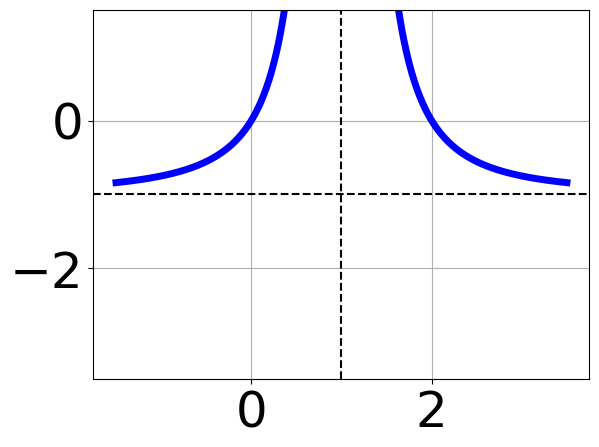
\includegraphics[width = 0.3\textwidth]{../Figures/rationalEquationToGraphCC.png}\item 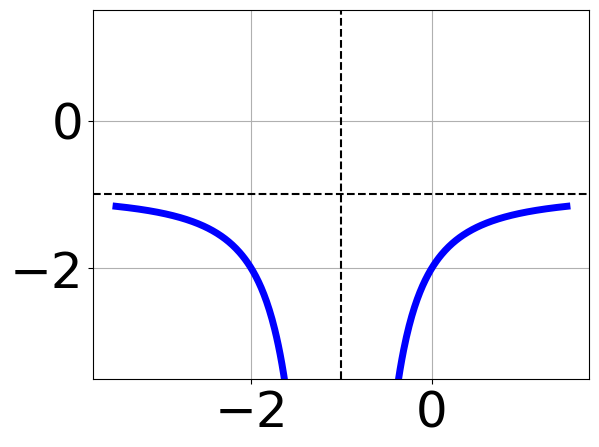
\includegraphics[width = 0.3\textwidth]{../Figures/rationalEquationToGraphDC.png}\end{multicols}\item None of the above.
\end{enumerate} }
\litem{
Choose the equation of the function graphed below.
\begin{center}
    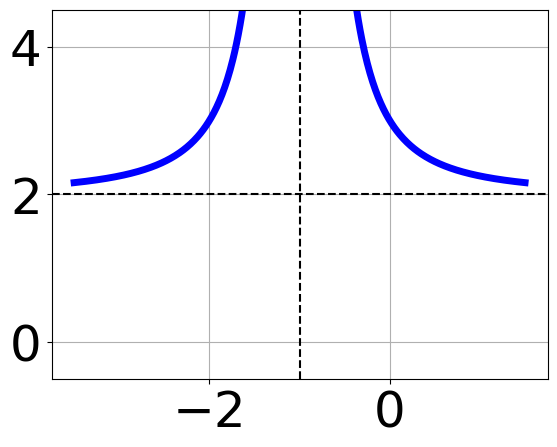
\includegraphics[width=0.5\textwidth]{../Figures/rationalGraphToEquationC.png}
\end{center}
\begin{enumerate}[label=\Alph*.]
\item \( f(x) = \frac{1}{(x + 1)^2} + 2 \)
\item \( f(x) = \frac{1}{x + 1} + 2 \)
\item \( f(x) = \frac{-1}{x - 1} + 2 \)
\item \( f(x) = \frac{-1}{(x - 1)^2} + 2 \)
\item \( \text{None of the above} \)

\end{enumerate} }
\litem{
Solve the rational equation below. Then, choose the interval(s) that the solution(s) belongs to.\[ \frac{7x}{-3x + 2} + \frac{-4x^{2}}{-15x^{2} -2 x + 8} = \frac{3}{5x + 4} \]\begin{enumerate}[label=\Alph*.]
\item \( x_1 \in [-0.23, 0.38] \text{ and } x_2 \in [-0.4,2.07] \)
\item \( x \in [-1.01,-0.56] \)
\item \( x \in [-1.6,-1.11] \)
\item \( x_1 \in [-0.23, 0.38] \text{ and } x_2 \in [-1.8,-1.25] \)
\item \( \text{All solutions lead to invalid or complex values in the equation.} \)

\end{enumerate} }
\litem{
Solve the rational equation below. Then, choose the interval(s) that the solution(s) belongs to.\[ \frac{-63}{63x -21} + 1 = \frac{-63}{63x -21} \]\begin{enumerate}[label=\Alph*.]
\item \( x_1 \in [-1.1, 0] \text{ and } x_2 \in [0.33,2.33] \)
\item \( x \in [-1.1,0] \)
\item \( x \in [0.33,2.33] \)
\item \( \text{All solutions lead to invalid or complex values in the equation.} \)
\item \( x_1 \in [-0.1, 0.6] \text{ and } x_2 \in [0.33,2.33] \)

\end{enumerate} }
\litem{
Choose the equation of the function graphed below.
\begin{center}
    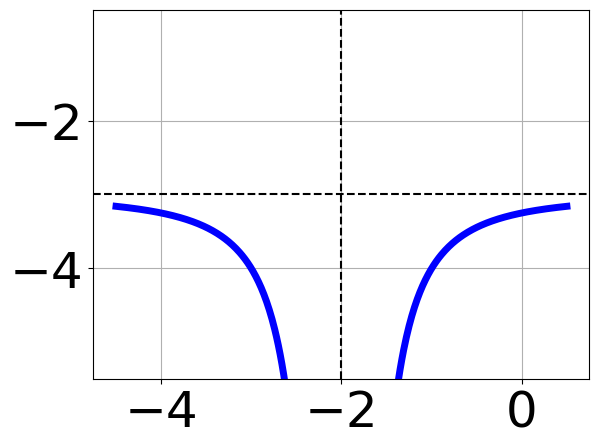
\includegraphics[width=0.5\textwidth]{../Figures/rationalGraphToEquationCopyC.png}
\end{center}
\begin{enumerate}[label=\Alph*.]
\item \( f(x) = \frac{1}{x + 2} - 3 \)
\item \( f(x) = \frac{-1}{(x - 2)^2} - 3 \)
\item \( f(x) = \frac{1}{(x + 2)^2} - 3 \)
\item \( f(x) = \frac{-1}{x - 2} - 3 \)
\item \( \text{None of the above} \)

\end{enumerate} }
\litem{
Solve the rational equation below. Then, choose the interval(s) that the solution(s) belongs to.\[ \frac{-5}{-6x + 2} + 8 = \frac{-6}{-12x + 4} \]\begin{enumerate}[label=\Alph*.]
\item \( x_1 \in [0.03, 0.67] \text{ and } x_2 \in [0.34,0.41] \)
\item \( x \in [0.29,1.29] \)
\item \( x_1 \in [-0.4, -0.35] \text{ and } x_2 \in [0.13,0.33] \)
\item \( \text{All solutions lead to invalid or complex values in the equation.} \)
\item \( x \in [-0.4,-0.35] \)

\end{enumerate} }
\litem{
Choose the graph of the equation below.\[ f(x) = \frac{-1}{x - 1} - 1 \]\begin{enumerate}[label=\Alph*.]
\begin{multicols}{2}\item 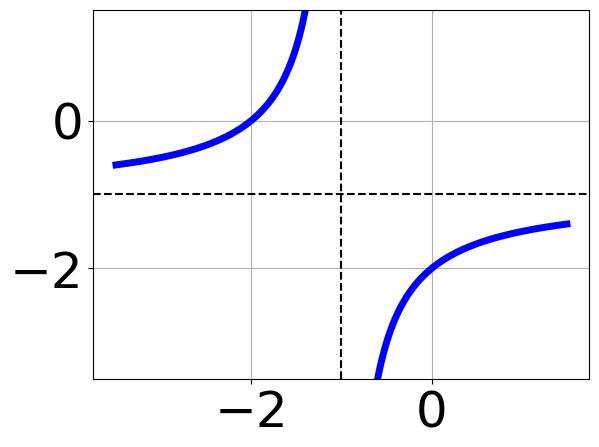
\includegraphics[width = 0.3\textwidth]{../Figures/rationalEquationToGraphCopyAC.png}\item 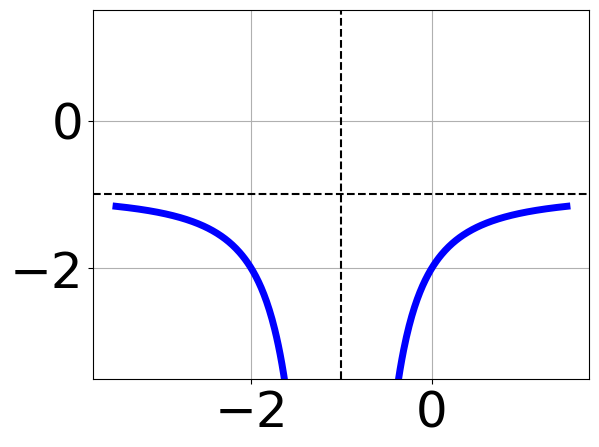
\includegraphics[width = 0.3\textwidth]{../Figures/rationalEquationToGraphCopyBC.png}\item 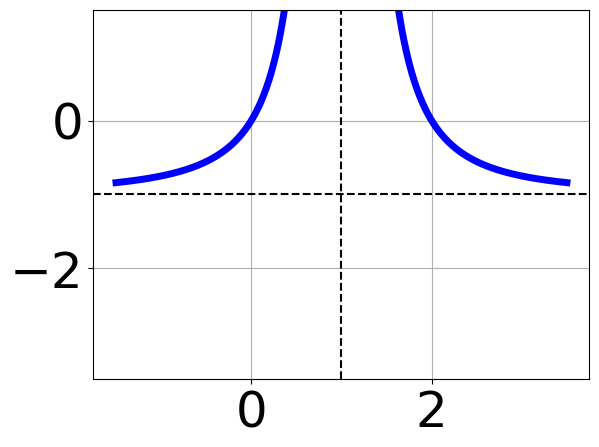
\includegraphics[width = 0.3\textwidth]{../Figures/rationalEquationToGraphCopyCC.png}\item 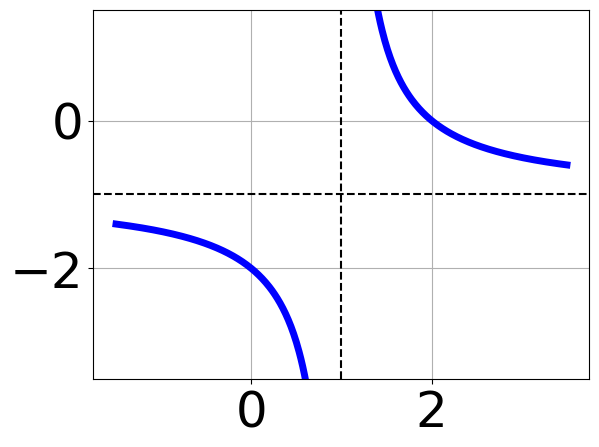
\includegraphics[width = 0.3\textwidth]{../Figures/rationalEquationToGraphCopyDC.png}\end{multicols}\item None of the above.
\end{enumerate} }
\litem{
Determine the domain of the function below.\[ f(x) = \frac{6}{12x^{2} -33 x + 18} \]\begin{enumerate}[label=\Alph*.]
\item \( \text{All Real numbers except } x = a, \text{ where } a \in [0.75, 1.75] \)
\item \( \text{All Real numbers.} \)
\item \( \text{All Real numbers except } x = a, \text{ where } a \in [11, 14] \)
\item \( \text{All Real numbers except } x = a \text{ and } x = b, \text{ where } a \in [11, 14] \text{ and } b \in [18, 20] \)
\item \( \text{All Real numbers except } x = a \text{ and } x = b, \text{ where } a \in [0.75, 1.75] \text{ and } b \in [2, 4] \)

\end{enumerate} }
\litem{
Determine the domain of the function below.\[ f(x) = \frac{6}{18x^{2} -6 x -12} \]\begin{enumerate}[label=\Alph*.]
\item \( \text{All Real numbers.} \)
\item \( \text{All Real numbers except } x = a, \text{ where } a \in [-1.67, 0.33] \)
\item \( \text{All Real numbers except } x = a \text{ and } x = b, \text{ where } a \in [-25, -21] \text{ and } b \in [5, 11] \)
\item \( \text{All Real numbers except } x = a, \text{ where } a \in [-25, -21] \)
\item \( \text{All Real numbers except } x = a \text{ and } x = b, \text{ where } a \in [-1.67, 0.33] \text{ and } b \in [0, 3] \)

\end{enumerate} }
\litem{
Solve the rational equation below. Then, choose the interval(s) that the solution(s) belongs to.\[ \frac{6x}{7x + 3} + \frac{-3x^{2}}{35x^{2} -27 x -18} = \frac{6}{5x -6} \]\begin{enumerate}[label=\Alph*.]
\item \( x \in [1.92,3.52] \)
\item \( x_1 \in [-0.41, 0.06] \text{ and } x_2 \in [1.1,6.1] \)
\item \( x_1 \in [-0.41, 0.06] \text{ and } x_2 \in [-6.43,0.57] \)
\item \( \text{All solutions lead to invalid or complex values in the equation.} \)
\item \( x \in [0.93,1.32] \)

\end{enumerate} }
\end{enumerate}

\end{document}